\section{Понятие защиты информации.}
\subsection{Общее представление о защите информации.}
Современные методы обработки, передачи и накопления информации с помощью информационный систем способствовали 
появлению угроз, связанных с возможностью потери, искажения и раскрытия данных, адресованных или принадлежащих 
конечным пользователям. Поэтому обеспечение информационной безопасности компьютерных систем и сетей становится 
одним из основных направлений в области информационных технологий.\cite{sh}

Словосочетание «информационная безопасность» в разных контекстах может иметь различный смысл. В Доктрине информационной
безопасности Российской Федерации термин «информационная безопасность» используется в глобальном смысле. Имеется в виду 
состояние защищенности национальных интересов в информационной сфере, определяемых совокупностью сбалансированных интересов 
личности, общества и государства. 

Под информационной безопасностью в узком смысле стоит понимать защищенность информации и поддерживающей инфраструктуры от 
случайных или преднамеренных воздействий естественного или искусственного характера, которые могут нанести неприемлемый ущерб 
субъектам информационных отношений, в том числе владельцам и пользователям информации и поддерживающей инфраструктуры. 

Таким образом, \textbf{защита информации} "---  это совокупность действий, направленных на обеспечение информационной безопасности.\cite{untuit}

Можно выделить несколько основных задач, решение которых в информационных системах и телекоммуникационных сетях обеспечивает 
защиту информации, а именно:
\begin{itemize}
    \item организация доступа к информации только допущенных к ней лиц;
    \item подтверждение истинности информации;
    \item защита от перехвата информации при передаче ее по каналам связи;
    \item защита от искажений и ввода ложной информации.
\end{itemize}
Защитить информацию "---  это значит:
\begin{itemize}
    \item обеспечить физическую целостность информации, т.е. не допустить искажений или уничтожения элементов информации;
    \item не допустить подмены (модификации) элементов информации при сохранении ее целостности;
    \item не допустить несанкционированного получения информации лицами или процессами, не имеющими на это соответствующих 
    полномочий;
    \item быть уверенным в том, что передаваемые (продаваемые) владельцем информации ресурсы будут использоваться только в 
    соответствии с обговоренными сторонами условиями.
\end{itemize}

\textbf{Угрозы информационной безопасности} "---  это оборотная сторона использования информационных технологий. Возвращаясь к вопросам 
терминологии, отметим, что термин «компьютерная безопасность» представляется нам слишком узким. Компьютеры "---  только одна из 
составляющих информационных систем, и хотя наше внимание будет сосредоточено в первую очередь на информации, которая 
хранится, обрабатывается и передается с помощью компьютеров, ее безопасность определяется всей совокупностью составляющих и, 
в первую очередь, самым слабым звеном, которым в подавляющем большинстве случаев оказывается человек (записавший, например, 
свой пароль на листке, прикреплённом к монитору). \cite{studfile}
\newpage
\subsection{Исторические этапы развития информационной безопасности.}
Методы и средства защиты информации в каждую историческую эпоху тесно связаны с уровнем развития науки и техники. Категории 
защищаемой информации определялись экономическими, политическими и военными интересами государства. Элементы защиты 
информации использовались с древнейших времён: известно, что тайнопись применяли ещё в Древнем Египте и Древнем Риме. По 
свидетельству Геродота, уже в V в. до н. э. применялось кодирование информации. Классическим примером одного из первых 
применений криптографии является так называемый «шифр Цезаря».\cite{urfu}
\begin{figure}[h]
    \centering
    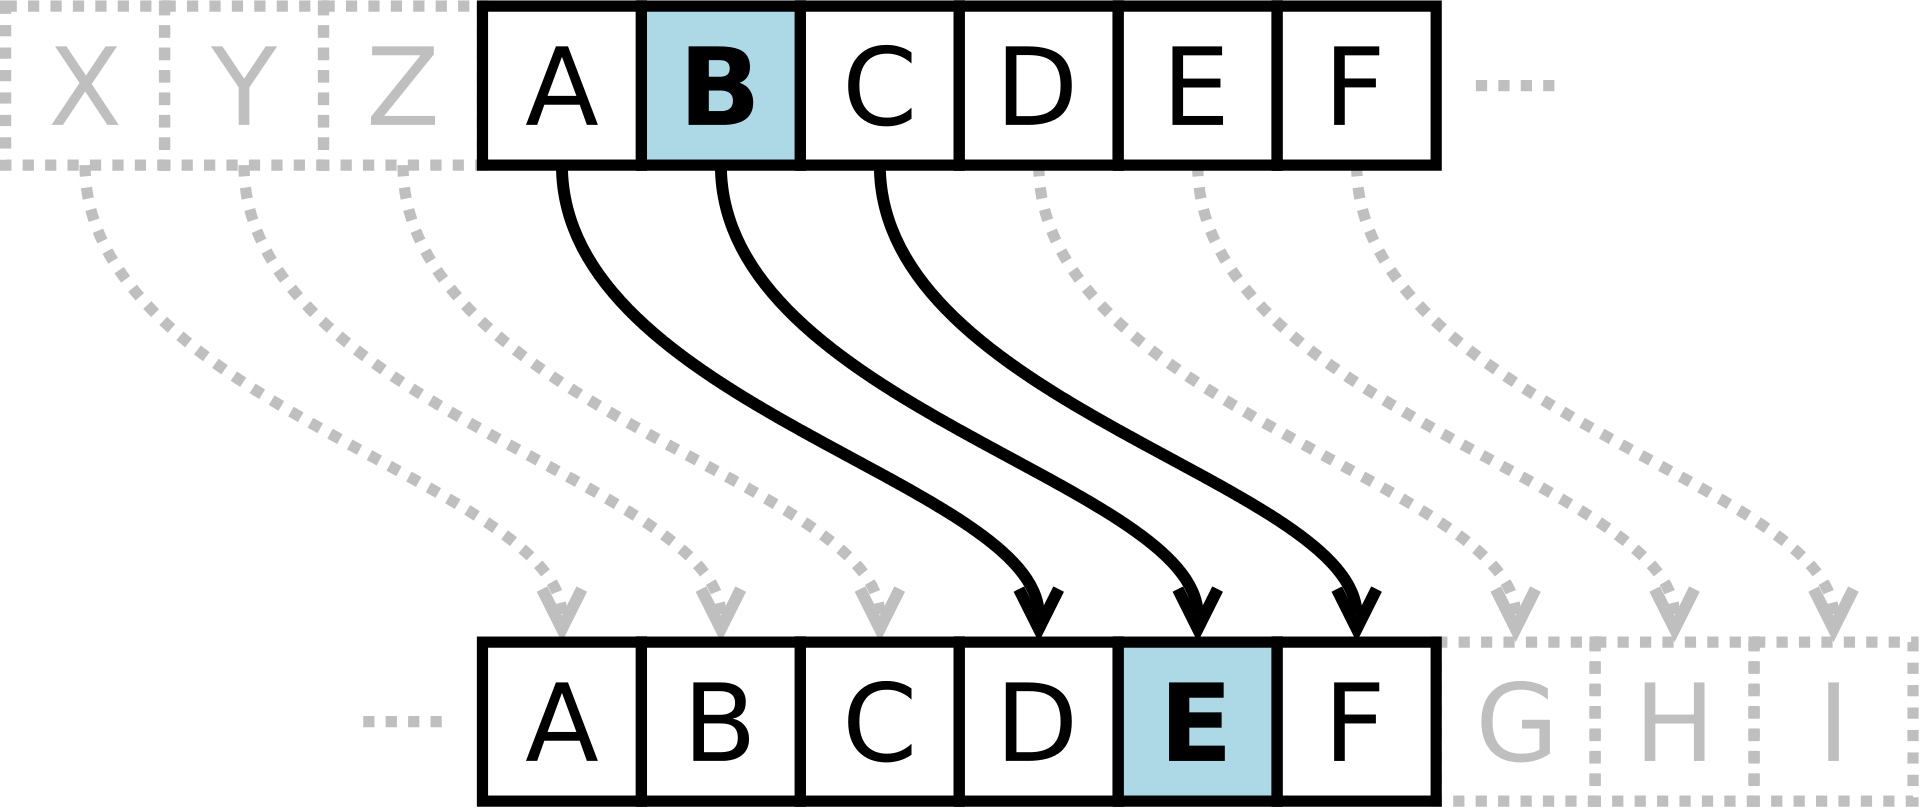
\includegraphics[width=0.5\textwidth]{pic/2.1.png}
    \caption{«шифр Цезаря»}
\end{figure}

Основоположником «шифра» в России является Иван Грозный, создавший «циферное отделение». В свою очередь, в 1702 году Пётр I 
учредил посольскую канцелярию, которая придумывала шифры и занималась расшифровкой текстов от иностранных послов.

\begin{figure}[h]
    \centering
    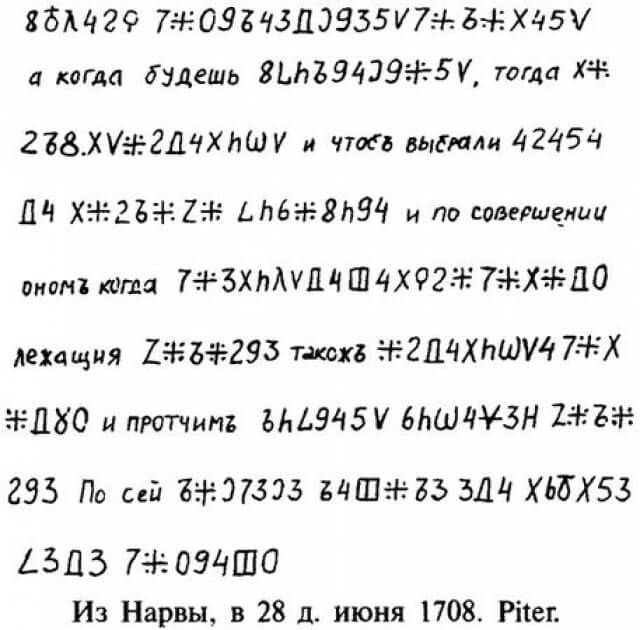
\includegraphics[width=0.5\textwidth]{pic/2.2.jpg}
    \caption{«шифр Петра I»}
\end{figure}

В следующем этапе развития методов защиты информации произошел значительный прорыв с появлением и широким распространением 
технических средств защиты, включая роторные машины. Одним из первых примеров таких машин была Enigma, созданная немецкими 
изобретателями Эдвардом Хеберном и Артуром Кирхом в 1917 году. Роторные системы были важным средством защиты конфиденциальной 
информации в то время, например во время Второй мировой войны такие системы, как Enigma (Германия), Sigaba (США), Турех 
(Великобритания), Red, Orange и Purple2 (Япония) были широко использованы. Однако только с развитием компьютеров в начале 
40-х годов стали возможны успешные крипто-атаки на роторные системы. В то же время, методы защиты от технических утечек 
информации совершенствовались, что способствовало развитию технической разведки государственными и коммерческими 
организациями.

С появлением первых компьютеров вместе с их развитием и интеграцией в общество, кодировка с использованием блочных шифров стала более распространенной и надежной альтернативой роторным системам из-за их высокой скорости обработки и передачи 
информации. Прорыв в области информационной безопасности случился в 1970-е годы с появлением первых вирусов и хакеров, что 
привело к необходимости разработки новых методов защиты, таких как антивирусное программное обеспечение, межсетевые экраны и 
системы обнаружения вторжений.

В 1977 году был принят стандарт шифрования DES в США, разработанный компанией IBM, который послужил основой для многих других 
моделей криптосистем по всему миру. С развитием интернета в 1990-е годы информационная безопасность стала более актуальной 
проблемой из-за появления новых угроз, таких как фишинг, спам и DDoS-атаки. Для противодействия этим угрозам были разработаны 
новые методы защиты, такие как шифрование данных, аутентификация пользователей и защита от DDoS.\cite{sforum}

На современном этапе развития общества информация выступает как форма собственности, и следовательно, имеет определенную 
ценность. Чтобы подчеркнуть роль информации в обществе, говорят об «информационном обществе», в отличие от предыдущей фазы 
развития общества "---  «индустриальном обществе». Начиная с 90-х гг. ХХ в. исследованиями в области информационной безопасности 
активно занимаются российские ученые. В.А. Герасименко разработал системно-концептуальный подход к обеспечению информационной 
безопасности автоматизированных систем обработки данных. А.А. Грушо и Е.Е. Тимонина представили доказательный подход к 
проблеме гарантированности защиты информации в компьютерной системе. А.А. Грушо в сферу исследований были введены новые виды 
скрытых каналов утечки информации, основывающихся на использовании статистических характеристик работы системы. С.П. 
Расторгуев и А.Ю. Щербаков разработали теорию разрушающих программных воздействий. А.Ю. Щербаковым также была разработана 
субъектно-объектная модель системы, на базе которой сформированы понятия информационных потоков и доступов в компьютерной 
системе. 

В настоящее время теория информационной безопасности продолжает развиваться. Появляются новые угрозы и вызовы, связанные с 
развитием информационных технологий. Это требует разработки новых методов и средств защиты информации.\cite{urfu}

\newpage
\subsection{Необходимость защиты информации.}
Бурное развитие средств вычислительной техники открыло перед человечеством непревзойденные возможности для автоматизации 
умственного труда, приведя к появлению многочисленных автоматизированных информационных и управляющих систем, а также к 
зарождению совершенно новых информационных технологий. Некоторые психологи считают, что человек разумный постепенно 
превращается в человека информационного.

Доступность вычислительной техники, особенно персональных компьютеров, привела к распространению компьютерной грамотности в 
широких кругах населения, что, естественно, привело к увеличению числа попыток незаконного вторжения в работу государственных 
и коммерческих автоматизированных систем - как с злым умыслом, так и чисто "из спортивного интереса". К сожалению, многие из 
таких попыток приводят к успеху и наносят значительный ущерб всем заинтересованным сторонам информационных отношений.

При анализе проблем, связанных с информационной безопасностью, следует учитывать специфику данной сферы. Он 
является составной частью информационных технологий, сферы, которая развивается с поразительной скоростью. Тут важны не 
только отдельные решения (законы, учебные курсы, программно-технические изделия), соответствующие современному уровню, но и 
механизмы создания новых решений, позволяющие им следовать темпу технического прогресса. К сожалению, существующая на 
сегодняшний день технология программирования не обеспечивает создание безупречных программ, что затрудняет быстрое развитие 
средств обеспечения информационной безопасности. Необходимо создавать надежные системы (информационной безопасности) с 
использованием ненадежных компонентов (программ). В принципе, это возможно, но требует соблюдения определенных архитектурных 
принципов и контроля за уровнем защищенности на протяжении всего жизненного цикла программы.

Увеличение числа атак "--- не самое страшное. Хуже то, что непрерывно обнаруживаются новые уязвимые места в программном 
обеспечении (связываемое с ограничениями современной технологии программирования) и, как следствие, возникают новые виды атак.

В этих условиях системы информационной безопасности должны быть способны противостоять различным атакам, как внешним, так и 
внутренним, автоматизированным и скоординированным. Иногда атаки длительны всего лишь доли секунды; порой поиск уязвимостей 
проводится медленно, растягивается на часы, так что подозрительная деятельность почти незаметна. Целью злоумышленников может 
быть нарушение всех аспектов информационной безопасности "---  доступности, целостности или конфиденциальности.\cite{biblio}
